\chapter{调试与性能分析}
\label{cp:debug}

\section{概述}

在Linux开发环境中,\textbf{调试与性能分析是系统开发和优化过程中至关重要的环节。}本实验围绕\textit{多种调试工具和性能分析技术展开},练习如何\textit{定位程序中的错误、优化性能瓶颈,并深入了解系统资源的使用情况}。\\

Linux系统的开放,使其拥有\textbf{丰富的调试和性能分析工具},这些工具\textit{各有其适用场景与优缺点},实验中会详细讨论并尝试应用这些工具。

\section{专用调试工具}

\subsection{使用GNU Debugger}

\textbf{GDB (GNU Debugger) 一般面向C/C++程序,是一个功能强大的调试工具。}通过命令行\textit{提供强大的调试能力,允许用户设置断点、单步执行、检查变量值、修改内存状态等}。实际上,我们在C/C++的学习中,已经对\textit{GDB}有所涉猎。\\

一般地,我们通过如\ref{listing:gdb}所示的方法,在C语言程序中启动\textit{GDB},并通过\texttt{run}命令执行程序。在程序运行过程中,我们可以通过\texttt{break}命令设置断点,通过\texttt{next}命令单步执行,通过\texttt{print}命令查看变量值,通过\texttt{watch}命令监视变量值等。\\

\begin{longlisting}
    \begin{minted}{bash}
# 有可能要先安装 gcc 和 gdb 工具
sudo apt install gcc gdb -y

# 用 echo 编写一个简单的 C 程序
echo '#include <stdio.h>
int main() {
    int a = 1;
    int b = 2;
    int c = a + b;
    printf("a + b = %d\n", c);
    return 0;
}' > test.c

# 编译 C 程序
# 其中 -g 选项表示生成调试信息,这样 GDB 才能正确调试
gcc -g test.c -o test
chmod +x test

# 启动 GDB 调试
gdb ./test

# 使用 list 命令可以查看源代码
(gdb) list
## 测试中的程序源码被打印

# 在 GDB 中执行 run 命令
(gdb) run
## 程序开始运行,输出 a + b = 3

# 可以使用 break (b), next (n), step (s), print (p), continue (c) 等命令在 run 后进行调试

# 设置断点为 main 函数
# 或者我们设置断点为 Line 4
(gdb) b main
## Breakpoint 1, main () at test.c:3
## 3           int a = 0;
(gdb) b 4
## Breakpoint 2 at 0x55555555515c: file test.c, line 4.

# 执行程序
(gdb) run
# 打印变量 a
(gdb) p a
## $1 = 0
(gdb) c
## Continuing.
## Breakpoint 2, main () at test.c:4
## 4           int b = 2;
# 此时再打印变量 a
(gdb) p a
## $2 = 1
(gdb) c
## Continuing.
## a + b = 3
## [Inferior 1 (process 16498) exited normally]

# 退出 GDB
(gdb) quit
    \end{minted}
    \caption{使用GDB调试C程序的示例}
    \label{listing:gdb}
\end{longlisting}

\subsection{使用LLVM Debugger}

\textbf{LLDB (LLVM Debugger) 也是一个功能强大的调试工具,面向C/C++程序。}与\textit{GDB}相比,是\textit{更为强大的替代工具,基于LLVM架构,启动速度更快,支持现代C++标准,尤其在调试C++项目时优势明显。}\\

\textit{LLDB}的使用方法与\textit{GDB}类似,如\ref{listing:lldb}所示。我们可以通过\texttt{lldb}命令启动\textit{LLDB},通过\texttt{run}命令执行程序,通过\texttt{breakpoint set}命令设置断点,通过\texttt{next}命令单步执行,通过\texttt{print}命令查看变量值等。\\

\begin{longlisting}
    \begin{minted}{bash}
# 有可能要先安装 clang 和 lldb 工具
sudo apt install clang lldb -y

# 依然用 echo 编写一个简单的 C 程序
echo '#include <stdio.h>
int main() {
    int a = 1;
    int b = 2;
    int c = a + b;
    printf("a + b = %d\n", c);
    return 0;
}' > test.c

# 编译 C 程序
clang -g test.c -o test
chmod +x test

# 启动 LLDB 调试
lldb ./test

# 使用 list 命令可以查看源代码
(lldb) list
## 测试中的程序源码被打印

# 在 LLDB 中执行 run 命令
(lldb) run
## 程序开始运行,输出 a + b = 3

# 类似的,可以使用 breakpoint set, next, step, print, continue 等命令在 run 后进行调试

# 设置断点为 main 函数
# 或者我们设置断点为 Line 4
(lldb) breakpoint set --name main
## Breakpoint 1: where = test`main, address = 0x0000000100000f80
(lldb) breakpoint set --file test.c --line 4
## Breakpoint 2: where = test`main + 20 at test.c:4, address = 0x0000000100000f94

# 执行程序
(lldb) run

# 打印变量 a
(lldb) print a
## (int) $0 = 0

# 继续执行
(lldb) continue

# 此时再打印变量 a
(lldb) print a
## (int) $1 = 1

# 继续执行
(lldb) continue
## a + b = 3
## Process 16498 exited with status = 0 (0x00000000)

# 退出 LLDB
(lldb) quit
    \end{minted}
    \caption{使用LLDB调试C程序的示例}
    \label{listing:lldb}
\end{longlisting}

\section{第三方日志系统}

\subsection{简介}

\textbf{第三方日志系统是一种记录程序运行状态的工具。}在实际开发中,\textit{对于复杂的应用程序,实时跟踪每个函数的执行情况非常困难,因此集成第三方日志系统成为调试的重要手段。}我们经常使用\textit{log4cpp}和\textit{spdlog}等日志库。\\

\subsection{spdlog的简单用例}

在C++程序中,我们使用\textit{spdlog}库来记录日志。如\ref{listing:spdlog}所示,我们可以通过\texttt{spdlog::info}、\texttt{spdlog::warn}、\texttt{spdlog::error}等方法记录不同级别的日志。\\

\begin{longlisting}
    \begin{minted}{cpp}
#include <spdlog/spdlog.h>

int main() {
    spdlog::info("Program started.");
    int a = 5;
    int b = 10;
    spdlog::debug("a = {}, b = {}", a, b);
    int c = a + b;
    spdlog::info("Result: {}", c);
    spdlog::warn("This is a warning!");
    spdlog::error("An error occurred!");
    return 0;
}
    \end{minted}
    \caption{使用spdlog记录日志的示例}
    \label{listing:spdlog}
\end{longlisting}

如此,可以做到\textbf{方便地与文件系统或控制台集成},并通过其\textit{异步日志记录功能,确保日志输出不会显著影响程序性能}。在复杂应用程序中,适当使用日志记录能够大幅度简化问题排查流程。\\

若要具体地使用\textit{spdlog},我们需要先安装\textit{spdlog}库,然后在\textit{CMakeLists.txt}\footnote{对CMake的具体介绍请见章节\ref{cp:meta}。}中添加如下内容:

\begin{longlisting}
    \begin{minted}{cmake}
find_package(spdlog REQUIRED)
target_link_libraries(${PROJECT_NAME} PRIVATE spdlog::spdlog)
    \end{minted}
    \label{listing:spdlog-cmake}
\end{longlisting}

\section{可视化调试工具}

\subsection{简介}

\textbf{STrace是一款强大的动态追踪工具},允许开发者\textit{在程序的各个执行点插入探针,从而捕捉系统调用、函数调用等底层信息}。而\textbf{Perfetto则专注于时间线可视化分析},能够将程序运行时的\textit{每个事件绘制成直观的图表,以帮助理解程序的执行顺序和时长。}譬如说,如果我们要调试一个多线程程序,使用\textit{Perfetto}可以非常方便地\textit{定位线程调度问题,分析哪部分代码导致了性能瓶颈或死锁。}

\subsection{STrace的简单用例}

\textbf{STrace}是一个\textit{Linux系统}下的\textbf{系统调用跟踪工具},我们可以通过\texttt{strace}命令来使用。如\ref{listing:strace}所示,我们可以通过\texttt{strace}命令跟踪程序的系统调用,从而了解程序的执行情况。\\

\begin{longlisting}
    \begin{minted}{bash}
# 使用 strace 跟踪程序
strace ./test
## 输出系统调用信息
    \end{minted}
    \caption{使用STrace跟踪C程序的示例}
    \label{listing:strace}
\end{longlisting}

当然,\texttt{strace}的功能远不止如此,我们可以通过\texttt{strace}命令的不同选项,来实现更多的功能。例如,我们可以通过\texttt{-c}选项统计系统调用的次数,通过\texttt{-t}选项显示时间戳,通过\texttt{-p}选项跟踪指定进程等。由于学习曲线过于陡峭,我们在此不再详细展开。

\subsection{Perfetto的简单用例}

\textbf{Perfetto}是一个\textit{Linux系统}下的\textbf{性能分析工具},我们可以通过\texttt{perfetto}命令来使用。如\ref{listing:perfetto}所示,我们可以通过\texttt{perfetto}命令启动\textit{Perfetto},并通过\texttt{UI}界面来查看程序的性能分析结果。\\

\textbf{perfetto是基于Chrome的Tracing实现},因此\textit{应该在具有图形界面的环境下使用。}

\section{内存泄漏检测与性能分析}

\subsection{概述}

\textbf{性能分析是系统开发过程中的重要环节},通过性能分析,我们可以\textit{找出程序中的性能瓶颈,优化程序的性能}。而\textbf{内存泄漏检测则是系统开发过程中的常见问题},通过内存泄漏检测,我们可以\textit{找出程序中的内存泄漏问题,避免程序的内存泄漏}。\\

\textbf{Valgrind和htop是资源监控与分析的核心工具}。\textit{Valgrind是Linux上用于内存分析的知名工具},能够帮助开发者检测内存泄漏、无效内存访问、未初始化变量使用等问题。\textit{htop则是实时资源监控工具},提供了一种直观的方式查看系统的CPU、内存、I/O等资源使用情况。

\subsection{体验Valgrind}

\textbf{Valgrind会生成一份详细的报告,指出每次内存分配和释放的情况,并指出潜在的内存问题。}对于C/C++程序,\textit{内存管理错误常常难以排查,Valgrind通过其动态内存分析能力,为开发者提供了极具价值的诊断信息。}除了内存分析,Valgrind还包含了一些其他工具,例如\textit{callgrind},用于分析程序的调用图和函数性能。\\

接下来,我们体验其\textbf{内存检测能力}与\textbf{函数测试能力}。请见代码\ref{listing:valgrind}。\\

\begin{longlisting}
    \begin{minted}{bash}
# 有可能要先安装 valgrind 工具
sudo apt install valgrind -y

# 对我们刚刚的C程序测试内存泄漏
valgrind --leak-check=full ./test

# 对我们刚刚的C程序测试函数调用链
valgrind --tool=callgrind ./test
    \end{minted}
    \caption{使用Valgrind检测C程序的示例}
    \label{listing:valgrind}
\end{longlisting}

具体执行结果见图\ref{fig:valgrind}。\\

\begin{figure}[!htbp]
    \centering
    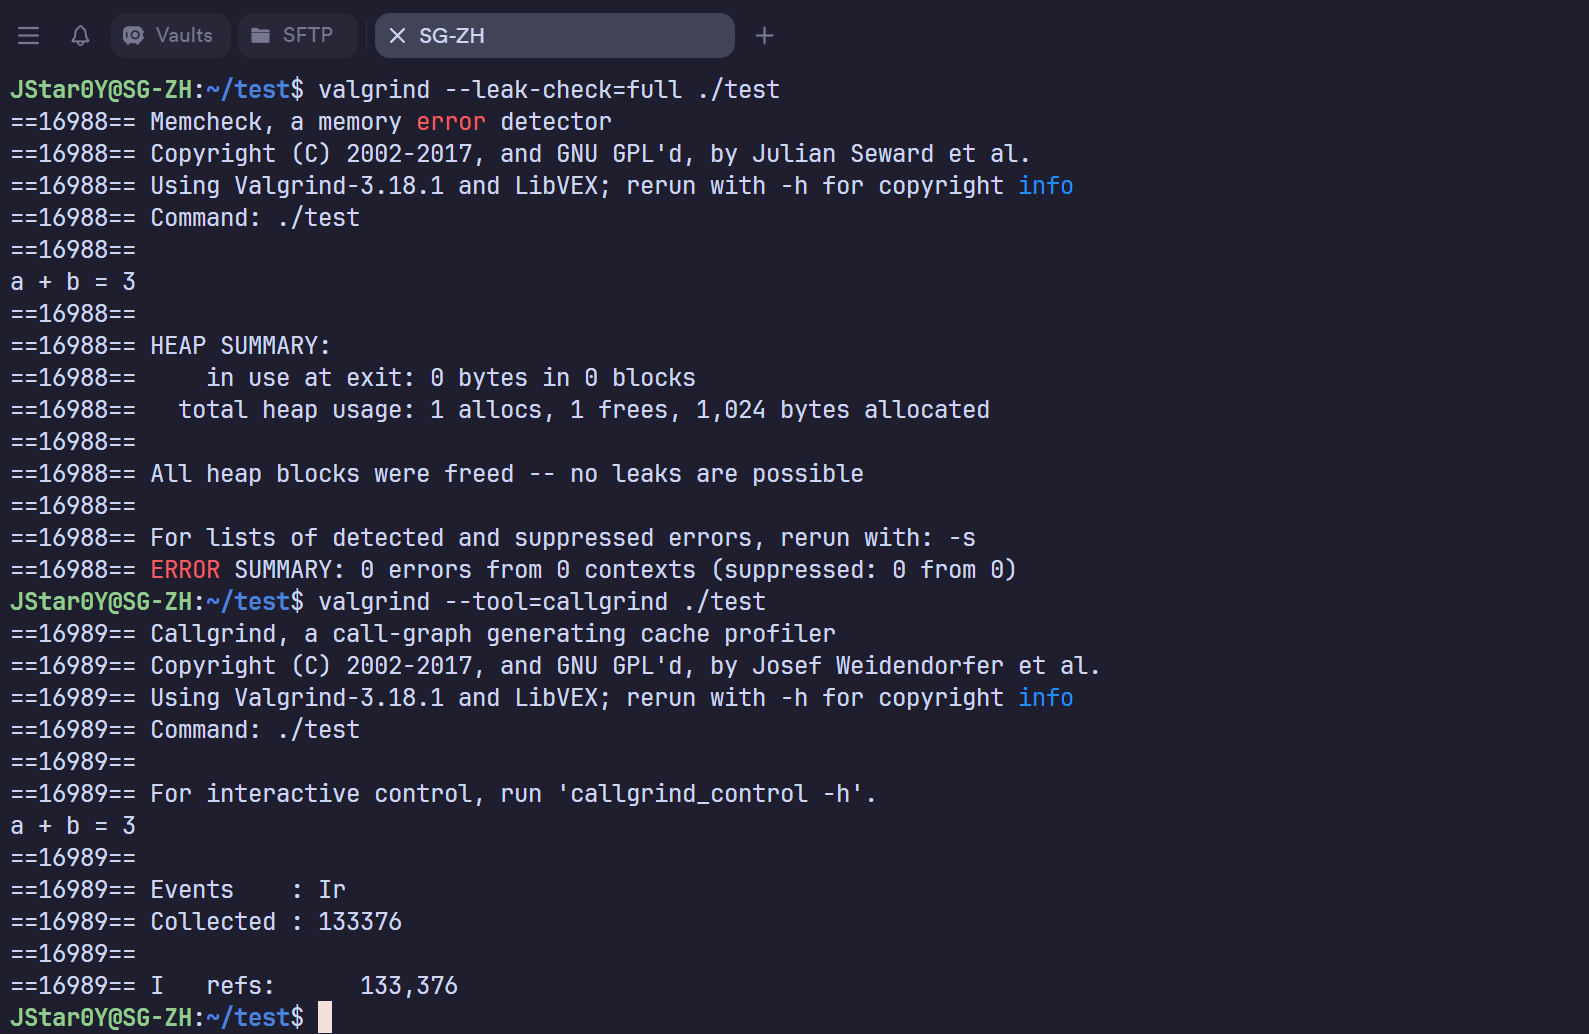
\includegraphics[width=0.8\textwidth]{Figures/valgrind.png}
    \caption{Valgrind的执行结果}
    \label{fig:valgrind}
\end{figure}